% =====================================================================
%  BayLearn — Module 2: Question Generation Subsystem
%  Graduation Project Report — Chapters 3, 4, 5 (Student A part)
%
%  HOW TO USE THIS FILE
%  --------------------
%  * It compiles standalone (pdflatex -> biber -> pdflatex x2) and
%    produces a self-contained PDF of Chapters 3-5 plus references.
%  * To paste into the team book: copy the three \chapter{...} blocks
%    (search for "CHAPTER 3", "CHAPTER 4", "CHAPTER 5"), and copy any
%    \usepackage lines your book preamble is missing, plus the
%    references entries from the embedded .bib (filecontents block).
%  * Citation style is APA (biblatex, style=apa).
%  * All figures are drawn in TikZ/pgfplots — NO external image files
%    are required.
% =====================================================================
\documentclass[12pt,a4paper]{report}

\usepackage[utf8]{inputenc}
\usepackage[T1]{fontenc}
\usepackage{lmodern}
\usepackage[margin=2.5cm]{geometry}
\usepackage{graphicx}
\usepackage{booktabs}
\usepackage{amsmath,amssymb}
\usepackage{listings}
\usepackage{xcolor}
\usepackage{microtype}
\usepackage{enumitem}
\usepackage{tikz}
\usepackage{pgfplots}
\pgfplotsset{compat=1.18}
\usetikzlibrary{shapes.geometric, arrows.meta, positioning, fit, backgrounds, calc}
\usepackage[hidelinks]{hyperref}

% ---- APA citations via biblatex -------------------------------------
\usepackage[style=apa, backend=biber]{biblatex}

% ---- Embedded bibliography (so the file is self-contained) ----------
\begin{filecontents*}{references.bib}
@inproceedings{sanh2019distilbert,
  author    = {Sanh, Victor and Debut, Lysandre and Chaumond, Julien and Wolf, Thomas},
  title     = {DistilBERT, a distilled version of BERT: smaller, faster, cheaper and lighter},
  booktitle = {Proceedings of the 5th Workshop on Energy Efficient Machine Learning (NeurIPS)},
  year      = {2019}
}
@inproceedings{devlin2019bert,
  author    = {Devlin, Jacob and Chang, Ming-Wei and Lee, Kenton and Toutanova, Kristina},
  title     = {BERT: Pre-training of Deep Bidirectional Transformers for Language Understanding},
  booktitle = {Proceedings of NAACL-HLT},
  pages     = {4171--4186},
  year      = {2019}
}
@inproceedings{lin2017focal,
  author    = {Lin, Tsung-Yi and Goyal, Priya and Girshick, Ross and He, Kaiming and Doll{\'a}r, Piotr},
  title     = {Focal Loss for Dense Object Detection},
  booktitle = {Proceedings of the IEEE International Conference on Computer Vision (ICCV)},
  pages     = {2980--2988},
  year      = {2017}
}
@inproceedings{reimers2019sbert,
  author    = {Reimers, Nils and Gurevych, Iryna},
  title     = {Sentence-BERT: Sentence Embeddings using Siamese BERT-Networks},
  booktitle = {Proceedings of EMNLP-IJCNLP},
  pages     = {3982--3992},
  year      = {2019}
}
@inproceedings{brown2020gpt3,
  author    = {Brown, Tom B. and others},
  title     = {Language Models are Few-Shot Learners},
  booktitle = {Advances in Neural Information Processing Systems (NeurIPS)},
  volume    = {33},
  pages     = {1877--1901},
  year      = {2020}
}
@inproceedings{zheng2023judge,
  author    = {Zheng, Lianmin and others},
  title     = {Judging LLM-as-a-Judge with MT-Bench and Chatbot Arena},
  booktitle = {Advances in Neural Information Processing Systems (NeurIPS)},
  year      = {2023}
}
@inproceedings{szegedy2016labelsmoothing,
  author    = {Szegedy, Christian and Vanhoucke, Vincent and Ioffe, Sergey and Shlens, Jon and Wojna, Zbigniew},
  title     = {Rethinking the Inception Architecture for Computer Vision},
  booktitle = {Proceedings of the IEEE Conference on Computer Vision and Pattern Recognition (CVPR)},
  pages     = {2818--2826},
  year      = {2016}
}
@inproceedings{loshchilov2017sgdr,
  author    = {Loshchilov, Ilya and Hutter, Frank},
  title     = {{SGDR}: Stochastic Gradient Descent with Warm Restarts},
  booktitle = {International Conference on Learning Representations (ICLR)},
  year      = {2017}
}
@inproceedings{loshchilov2019adamw,
  author    = {Loshchilov, Ilya and Hutter, Frank},
  title     = {Decoupled Weight Decay Regularization},
  booktitle = {International Conference on Learning Representations (ICLR)},
  year      = {2019}
}
@book{anderson2001revised,
  author    = {Anderson, Lorin W. and Krathwohl, David R.},
  title     = {A Taxonomy for Learning, Teaching, and Assessing: A Revision of Bloom's Taxonomy of Educational Objectives},
  publisher = {Longman},
  year      = {2001}
}
@book{bloom1956taxonomy,
  author    = {Bloom, Benjamin S.},
  title     = {Taxonomy of Educational Objectives: The Classification of Educational Goals},
  publisher = {Longmans, Green},
  year      = {1956}
}
@inproceedings{lewis2020rag,
  author    = {Lewis, Patrick and others},
  title     = {Retrieval-Augmented Generation for Knowledge-Intensive NLP Tasks},
  booktitle = {Advances in Neural Information Processing Systems (NeurIPS)},
  year      = {2020}
}
@inproceedings{scaria2024aeqg,
  author    = {Scaria, Nicy and Chenna, Suman Dowlagar and Subramani, Deepak},
  title     = {Automated Educational Question Generation at Different Bloom's Skill Levels Using Large Language Models},
  booktitle = {Artificial Intelligence in Education (AIED)},
  year      = {2024}
}
@article{wolf2020transformers,
  author    = {Wolf, Thomas and others},
  title     = {Transformers: State-of-the-Art Natural Language Processing},
  journal   = {Proceedings of EMNLP: System Demonstrations},
  pages     = {38--45},
  year      = {2020}
}
@inproceedings{maity2025icl,
  author    = {Maity, Subhankar and Deroy, Aniket and Sarkar, Sudeshna},
  title     = {Leveraging In-Context Learning and Retrieval-Augmented Generation for Automatic Question Generation in Educational Domains},
  booktitle = {Proceedings of the 16th Meeting of the Forum for Information Retrieval Evaluation (FIRE)},
  year      = {2025}
}
@article{kumar2025automated,
  author    = {Kumar, Ramya and Gulwani, Dhruv and Singh, Sonit},
  title     = {Automated Analysis of Learning Outcomes and Exam Questions Based on Bloom's Taxonomy},
  journal   = {arXiv preprint arXiv:2511.10903},
  year      = {2025}
}
@inproceedings{duongtrung2024bloomllm,
  author    = {Duong-Trung, Nghia and others},
  title     = {BloomLLM: Large Language Models-Based Question Generation Combining Supervised Fine-Tuning and Bloom's Taxonomy},
  booktitle = {European Conference on Technology Enhanced Learning (EC-TEL)},
  year      = {2024}
}
@article{mohammed2020question,
  author    = {Mohammed, Manal and Omar, Nazlia},
  title     = {Question classification based on Bloom's taxonomy cognitive domain using modified TF-IDF and word2vec},
  journal   = {PLOS ONE},
  volume    = {15},
  number    = {3},
  pages     = {e0230442},
  year      = {2020}
}
@misc{lau2022bloombert,
  author       = {Lau, Ryan Qian Feng},
  title        = {BloomBERT: A Task Classification Framework Based on Bloom's Taxonomy},
  howpublished = {Project report and source code},
  year         = {2022}
}
% --- PLACEHOLDERS: replace with the exact references you intend ---
@misc{angelPLACEHOLDER,
  author       = {Angel, [AUTHORS]},
  title        = {[FULL TITLE OF THE ``Angel'' BLOOM-AWARE GENERATION PAPER]},
  howpublished = {[VENUE]},
  year         = {[YEAR]}
}
@misc{zamanPLACEHOLDER,
  author       = {Zaman, [AUTHORS]},
  title        = {[FULL TITLE / DATASET NAME OF THE ZAMAN BLOOM-LEVEL WORK]},
  howpublished = {[VENUE OR DATA REPOSITORY]},
  year         = {[YEAR]}
}
\end{filecontents*}
\addbibresource{references.bib}

% ---- listings style -------------------------------------------------
\definecolor{codebg}{rgb}{0.97,0.97,0.97}
\lstset{
  basicstyle=\ttfamily\footnotesize,
  backgroundcolor=\color{codebg},
  breaklines=true,
  frame=single,
  captionpos=b,
  showstringspaces=false,
  numbers=left,
  numberstyle=\tiny\color{gray}
}

% ---- chapters start at 3 to mirror the team book --------------------
\setcounter{chapter}{2}

\begin{document}

% =====================================================================
% CHAPTER 3 — LITERATURE SURVEY
% =====================================================================
\chapter{Literature Survey}

This chapter provides the technical background required to understand the
Question Generation subsystem of BayLearn (Module~2). The subsystem couples a
fine-tuned difficulty classifier, a retrieval-augmented few-shot generation
pipeline, and an automatic evaluation protocol. Accordingly, Section~3.1 reviews
Bloom's taxonomy as a model of cognitive difficulty and the transformer-based
text classification that operationalises it. Section~3.2 reviews in-context
learning and retrieval augmentation for controllable text generation.
Section~3.3 gives a short comparative review of recent work on automated
question generation. Section~3.4 states the approach adopted in this project and
justifies each design choice.

\section{Background on Cognitive Difficulty Modelling and Text Classification}

\subsection{Bloom's Taxonomy as a Difficulty Signal}
Bloom's taxonomy \parencite{bloom1956taxonomy}, later revised by
\textcite{anderson2001revised}, organises learning objectives along six
increasing levels of cognitive demand: \emph{Remember}, \emph{Understand},
\emph{Apply}, \emph{Analyze}, \emph{Evaluate}, and \emph{Create}. Each level is
characterised by typical action verbs (e.g.\ ``define'' for Remember, ``compare''
for Analyze, ``justify'' for Evaluate). In an adaptive-learning setting the
taxonomy is attractive because it provides a principled, pedagogically grounded
ordinal scale of difficulty that an upstream policy can request and a downstream
component can verify.

Because the downstream reinforcement-learning controller in BayLearn consumes a
three-level difficulty signal, this project collapses the six Bloom levels into
three buckets: \emph{easy} (Remember, Understand), \emph{medium} (Apply,
Analyze), and \emph{hard} (Evaluate, Create). This reduces label sparsity in the
two highest categories while preserving the ordinal structure that matters for
adaptive selection.

\subsection{Transformer Encoders and DistilBERT}
BERT \parencite{devlin2019bert} introduced bidirectional transformer
pre-training that produces contextual token representations transferable to
downstream tasks through fine-tuning. DistilBERT \parencite{sanh2019distilbert}
applies knowledge distillation to compress BERT into a six-layer student model
that retains roughly 97\% of BERT's language-understanding performance while
being about 40\% smaller and 60\% faster. For a classification task that must run
as an inline verifier inside a latency-sensitive generation pipeline, this
speed/quality trade-off makes DistilBERT a strong backbone.

A well-established empirical observation about BERT-family encoders is that lower
layers capture surface and syntactic regularities while upper layers capture
sentence-level semantics and task-specific abstractions. This motivates partial
fine-tuning: freezing lower layers preserves general linguistic competence
learned from large corpora, while unfreezing only the upper layers adapts the
model to the target task without catastrophically overwriting pre-trained
knowledge on a comparatively small dataset.

One detail that turns out to matter in practice is how the per-token encoder
output is reduced to a single vector before the classification head. The default
choice in DistilBERT sequence classification is to read the representation of the
first token. An alternative, common in sentence-embedding work, is mean pooling:
averaging the hidden states of all (non-padding) tokens. Mean pooling spreads the
signal across the whole sentence rather than concentrating it in one position,
which can help on longer, syntactically richer questions. Both options are
cheap, so the sensible thing is to treat the pooling strategy as one more knob to
test rather than to assume one is better; Chapter~5 reports what we found.

\subsection{Class Imbalance and the Focal Loss}
Educational question corpora are heavily skewed towards lower cognitive levels:
recall and comprehension questions vastly outnumber evaluation and creation
questions. Standard cross-entropy treats all examples equally and is dominated by
the majority class. The focal loss \parencite{lin2017focal} addresses this by
multiplying the cross-entropy of each example by a modulating factor
$(1-p_t)^{\gamma}$, where $p_t$ is the model's predicted probability for the true
class and $\gamma \ge 0$ is a focusing parameter. Well-classified examples
(high $p_t$) are down-weighted, concentrating gradient on hard, uncertain
examples near decision boundaries. Combined with inverse-frequency class
weighting, the focal loss is a natural fit for the imbalanced three-level Bloom
problem.

Two further regularisation techniques are relevant. Label smoothing
\parencite{szegedy2016labelsmoothing} replaces one-hot targets with a softened
distribution, discouraging over-confident predictions on noisy labels. Cosine
learning-rate scheduling \parencite{loshchilov2017sgdr}, together with the
decoupled weight decay of AdamW \parencite{loshchilov2019adamw}, provides a
smooth annealing schedule that can improve late-training stability.

\section{Background on Few-Shot Generation and Retrieval Augmentation}

\subsection{In-Context Learning and the Idea We Borrowed}
A large language model can pick up a task from a few worked examples placed in
its prompt, without any change to its weights. This behaviour, in-context
learning (ICL), was popularised by \textcite{brown2020gpt3}. What an example
``teaches'' depends entirely on what it demonstrates. Show the model three short
recall questions and it will tend to write short recall questions; show it three
multi-step analysis questions and the output shifts accordingly. The examples are
not just illustrations of the task---they are a soft instruction about the shape
of the answer.

The specific starting point for our generation design is the work of
\textcite{maity2025icl}, who study automatic question generation in the
educational domain. Their central observation is that a bare prompt often yields
questions that drift away from the source material, and that two ingredients fix
much of this: retrieval, to keep the generator anchored to real passages, and a
small set of in-context examples, to lift question quality. Their best system, a
hybrid, simply combines the two---retrieved context plus few-shot
demonstrations---and they report that this beats either ingredient alone under
both automatic and human evaluation.

We took that core idea---retrieval for grounding, few-shot examples for
quality---and adapted it to a requirement their paper does not address:
\emph{difficulty control}. In their setup the few-shot examples are there to make
questions better in general; there is no notion of asking for an easy question
versus a hard one. Our downstream controller, by contrast, asks for a specific
difficulty level, so the examples have to do a second job. We therefore changed
what gets retrieved. Instead of selecting demonstrations purely by topical
similarity, we first restrict the candidate pool to the requested difficulty
level and only then rank by similarity. In effect the example bank is indexed by
difficulty, and the retrieved demonstrations carry both ``this is the kind of
topic'' and ``this is the kind of difficulty'' at once. We also added a component
that has no counterpart in their pipeline: an independent, trained classifier
that checks the difficulty of every generated question after the fact, which we
describe in the next chapter.

\subsection{Retrieval-Augmented Generation and Dense Retrieval}
Retrieval-augmented generation (RAG) \parencite{lewis2020rag} conditions the
generator on passages pulled from an external store, so the output is tied to
real content instead of whatever the model happens to remember. Our pipeline uses
two retrievals that play different roles. The first is ordinary RAG over the
student's own material, and it fixes the \emph{content} of a question. The second
is retrieval over the example bank, and it fixes the \emph{form}---the difficulty
and phrasing the question should take. Keeping these separate is deliberate: we
want the demonstrations to nudge style and cognitive level without dragging in
content from unrelated topics.

Both retrievals rest on dense sentence embeddings. We use a Sentence-BERT
bi-encoder \parencite{reimers2019sbert}, which is trained so that sentences with
similar meaning land near each other in vector space. Once every question in the
bank is embedded and the vectors are length-normalised, ranking by relevance
reduces to a dot product, which is what makes online retrieval over tens of
thousands of entries effectively free.

\subsection{LLM-as-a-Judge Evaluation}
Surface metrics such as $n$-gram overlap correlate poorly with how a human would
rate a generated question, so we needed a better yardstick. The
LLM-as-a-judge approach \parencite{zheng2023judge} uses a strong model to compare
candidate outputs, and prior work shows it tracks human preference closely
provided the comparison is blinded and the presentation order is randomised to
cancel position bias. We use exactly this protocol to ask a direct question---are
the questions written with the difficulty-aligned example bank actually better
than those written without it?---and report the result alongside the
classifier-based difficulty metric in Chapter~5.

\section{Comparative Study of Previous Work}
Our subsystem sits at the meeting point of three lines of research: generating
questions at a chosen Bloom level, using retrieval and in-context examples to
improve question generation, and classifying the Bloom level of a question.
Reviewing the three together makes it clear where our contribution lives, because
no single prior line does all of what we need.

\subsection{Bloom-Aware Question Generation}
The first line conditions a generator on a target cognitive level.
\textcite{scaria2024aeqg} prompt large language models to produce questions at a
specified Bloom level and check alignment with both human raters and an automatic
classifier; their headline finding is that explicit level conditioning helps, but
the upper levels---evaluation and creation---stay the hardest to hit reliably.
BloomLLM \parencite{duongtrung2024bloomllm} pushes further by fine-tuning a model
specifically to emit questions at requested Bloom levels, trading the flexibility
of prompting for tighter control at the cost of a training stage and a labelled
generation corpus. A third strand
\parencite{angelPLACEHOLDER}\,\textbf{[CITATION NEEDED: confirm the ``Angel''
reference]} approaches Bloom-aware generation from a complementary angle. The
shared limitation across this group is that the difficulty of a generated
question is taken largely on trust: it is either the level the model was asked
for or a level a human annotated afterwards, with no independent automatic check
inside the loop.

\subsection{In-Context Learning and Retrieval for Question Generation}
The second line is about \emph{how} to prompt rather than \emph{what} level to
target. \textcite{maity2025icl} combine retrieval and few-shot demonstrations and
show the pairing produces more on-context, pedagogically sounder questions than
either piece alone. Their work is the direct ancestor of our generation design.
The gap, from our point of view, is that difficulty never enters their selection
of demonstrations---examples are chosen to raise quality, not to land a requested
level. Our adaptation keeps their retrieval-plus-ICL skeleton but makes the
target difficulty the primary retrieval key, so the same machinery that improves
quality also steers cognitive level.

\subsection{Bloom-Level Classification}
The third line treats Bloom level as a text-classification target in its own
right. Early work such as \textcite{mohammed2020question} pairs hand-engineered
features (modified TF--IDF, word2vec) with classical classifiers. BloomBERT
\parencite{lau2022bloombert} moves to a fine-tuned DistilBERT and is the closest
methodological relative of our classifier. A recent and instructive study by
\textcite{kumar2025automated} benchmarks the whole spectrum---classical models,
recurrent networks, transformers, and zero-shot LLMs---on a 600-sentence Bloom
corpus, and finds that an SVM with augmentation tops the table at about 94\%
while the deep models overfit badly and zero-shot LLMs land around 72--73\%.
That result is a warning more than a recipe: it says transformers struggle to
beat simple baselines \emph{when the labelled data is tiny}. Earlier
classification efforts built on small course-specific sets---including the Zaman
corpus \parencite{zamanPLACEHOLDER}\,\textbf{[CITATION NEEDED: confirm the Zaman
reference]}, which we examined and ultimately set aside because it was too small
to fine-tune a transformer on---run into the same wall.

\subsection{The Two Gaps We Address}
Reading the three groups together points to two concrete openings, each tied to a
specific weakness above.

\textbf{Gap 1 --- difficulty is asserted, not verified.} The generation papers in
the first group, and the hybrid pipeline of \textcite{maity2025icl} in the
second, have no independent component that confirms a finished question is
actually at the requested level. We close this by putting a separately trained
DistilBERT classifier in the loop as a verifier, so every generated question
carries a second opinion on its difficulty.

\textbf{Gap 2 --- small data sinks transformer classifiers.} The benchmark of
\textcite{kumar2025automated}, and the fate of small sets like the Zaman corpus,
show that a fine-tuned transformer needs a substantial labelled corpus to be
worth the trouble. Our answer is on the data side: rather than reuse a few
hundred labelled questions, we assemble a large educator-labelled corpus (the SRM
Valliammai Engineering College question banks, mapped to three difficulty levels)
so that fine-tuning a DistilBERT classifier is actually justified. The dataset
engineering that this required is described in Chapter~4.

\section{Implemented Approach}
Putting the two gaps together gives the shape of our system. We need a generator
that can be steered to a difficulty level (from the second research line), a way
to confirm it actually hit that level (Gap~1), and enough labelled data for the
confirming classifier to be trustworthy (Gap~2). Three components follow from
this.

The first is the difficulty classifier we call BloomBERT: a DistilBERT model
fine-tuned on the large educator-labelled corpus to predict easy, medium, or
hard. We chose DistilBERT rather than full BERT because the model runs on every
generated question and speed matters; we used focal loss with inverse-frequency
weighting because the hard class is rare and plain cross-entropy ignores it; and
we froze the lower layers because the corpus, while large, is still small next to
what DistilBERT saw in pre-training, and we did not want to erase that. The
classifier does double duty---it labels the example bank offline, and it verifies
generated questions online.

The second is the example bank itself: questions from the SRM corpus and a
hand-written Operating-Systems set, each embedded once with Sentence-BERT and
stored next to its vector. At generation time we filter to the requested
difficulty, rank the survivors by similarity to the topic, and drop the top few
into the prompt as worked examples. This is where our adaptation of
\textcite{maity2025icl} lives: their examples improve quality, ours improve
quality \emph{and} pin down difficulty.

The third is the evaluation. Because a single automatic number rarely tells the
whole story---and because our own classifier is one of the things under test---we
pair the classifier's difficulty-match rate with a blinded LLM-as-a-judge
comparison of questions written with and without the bank. The reasoning behind
each of these choices is worked out in Chapter~4, and Chapter~5 reports whether
they held up.

% =====================================================================
% CHAPTER 4 — SYSTEM DESIGN AND ARCHITECTURE
% =====================================================================
\chapter{System Design and Architecture}

This chapter describes the design of the Question Generation subsystem in full
detail, proceeding from the overall data flow to each fine-grained component. The
discussion is organised so that an interested reader could reconstruct the
subsystem. Section~4.1 states the overview and assumptions; Section~4.2 presents
the block diagram and end-to-end flow; Sections~4.3 and~4.4 describe the two
coarse modules---the BloomBERT difficulty classifier and the few-shot generation
pipeline---together with their decomposition and design constraints.

\section{Overview and Assumptions}
The subsystem receives a difficulty-conditioned request and the student's study
material, and returns questions that are (i) grounded in that material,
(ii) aligned to the requested difficulty, and (iii) verified by an independent
classifier. The following assumptions frame the design:
\begin{itemize}[leftmargin=*]
  \item The downstream controller specifies difficulty on a three-level scale
  (easy/medium/hard); the six Bloom levels are mapped onto these three buckets.
  \item Study material has already been ingested and is retrievable as text
  chunks by an upstream RAG component; the subsystem consumes chunks rather than
  raw documents.
  \item Text generation is delegated to a hosted large language model accessed
  through an API; the subsystem owns the prompting, retrieval, and verification
  logic, not the generator's weights.
  \item Embeddings for the example bank are computed once, offline, and cached;
  online cost is limited to a single query embedding plus a dot product.
\end{itemize}

\section{System Architecture}

\subsection{Block Diagram}
Figure~\ref{fig:pipeline} shows the end-to-end flow. A request specifying the
concept, difficulty, and question type enters the pipeline. Relevant content
chunks are retrieved from the student's material. In parallel, the example bank
is queried for difficulty-aligned demonstrations. A prompt is assembled from the
Bloom guidance, the retrieved demonstrations, and the content chunks, and sent to
the generator. Each generated question is then classified by BloomBERT; if too
many questions miss the requested level, a single bounded regeneration is
triggered. Verified questions, annotated with their predicted level and
confidence, are returned.

\begin{figure}[ht]
\centering
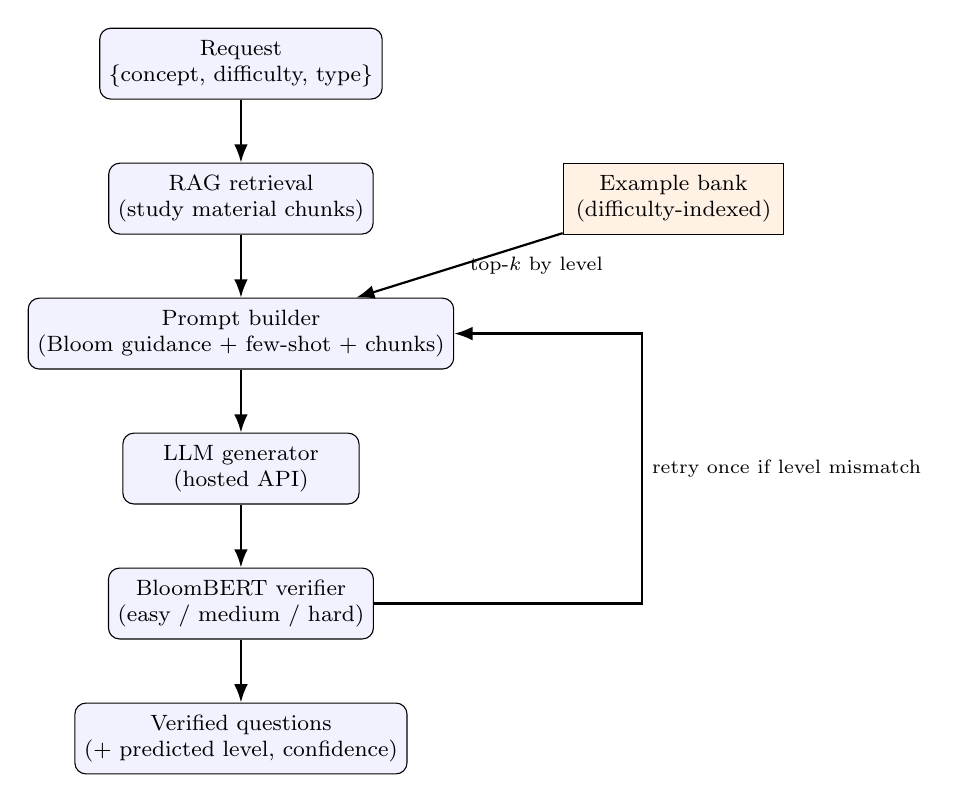
\begin{tikzpicture}[
  node distance=8mm and 12mm,
  box/.style={draw, rounded corners, align=center, minimum height=9mm,
              minimum width=30mm, font=\footnotesize, fill=blue!5},
  store/.style={draw, align=center, minimum height=9mm, minimum width=28mm,
                font=\footnotesize, fill=orange!10},
  arr/.style={-{Latex}, thick}
]
\node[box] (req) {Request\\\{concept, difficulty, type\}};
\node[box, below=of req] (rag) {RAG retrieval\\(study material chunks)};
\node[store, right=24mm of rag] (bank) {Example bank\\(difficulty-indexed)};
\node[box, below=of rag] (prompt) {Prompt builder\\(Bloom guidance + few-shot + chunks)};
\node[box, below=of prompt] (llm) {LLM generator\\(hosted API)};
\node[box, below=of llm] (clf) {BloomBERT verifier\\(easy / medium / hard)};
\node[box, below=of clf] (out) {Verified questions\\(+ predicted level, confidence)};

\draw[arr] (req) -- (rag);
\draw[arr] (rag) -- (prompt);
\draw[arr] (bank) -- node[right, font=\scriptsize]{top-$k$ by level} (prompt);
\draw[arr] (prompt) -- (llm);
\draw[arr] (llm) -- (clf);
\draw[arr] (clf) -- (out);
\draw[arr] (clf.east) -- ++(34mm,0) |- node[pos=0.25,right,font=\scriptsize]{retry once if level mismatch} (prompt.east);
\end{tikzpicture}
\caption{End-to-end architecture of the Question Generation subsystem. Solid
arrows show the forward path; the right-hand feedback arrow shows the bounded
single regeneration triggered when the verifier detects difficulty drift.}
\label{fig:pipeline}
\end{figure}

\section{Module 1: BloomBERT Difficulty Classifier}

\subsection{Functional Description}
BloomBERT maps a question string to one of three difficulty classes. It is built
on \texttt{distilbert-base-uncased} with a classification head, and serves two
roles: offline, it labels every entry of the example bank so that retrieval can
be keyed by difficulty; online, it verifies the difficulty of each generated
question and triggers regeneration on drift.

\subsection{Modular Decomposition}
The classifier pipeline decomposes into:
\begin{itemize}[leftmargin=*]
  \item \textbf{Data assembly.} A large educator-labelled question bank (the SRM
  Valliammai Engineering College public question banks) is parsed; each question
  carries an explicit Bloom level which is mapped to easy/medium/hard. The
  combined corpus is de-duplicated and split into train/validation/test
  partitions in an 80/10/10 ratio.
  \item \textbf{Tokenisation.} Questions are tokenised with the HuggingFace
  Transformers DistilBERT WordPiece tokenizer
  \parencite{wolf2020transformers} to a maximum length of 128 tokens.
  \item \textbf{Backbone with partial fine-tuning.} The embedding layer and the
  lower transformer layers are frozen; only the top transformer layers and the
  classification head are trainable.
  \item \textbf{Loss.} Inverse-frequency--weighted focal loss
  (Section~4.3.4) addresses the strong class imbalance.
  \item \textbf{Optimisation.} AdamW with layer-wise learning-rate decay, linear
  warmup, mixed-precision training, and best-checkpoint selection by validation
  macro-F1.
\end{itemize}

\subsection{Design Constraints}
Three constraints shaped the design. First, \emph{class imbalance}: the hard
class is an order of magnitude smaller than the easy class, so plain
cross-entropy under-serves it; the loss must explicitly compensate. Second,
\emph{limited in-domain data and catastrophic forgetting}: fully fine-tuning all
layers on a comparatively small corpus risks overwriting useful pre-trained
representations, so only upper layers are unfrozen. Third, \emph{inference
latency}: because the classifier runs inline on every generated question,
DistilBERT (rather than full BERT) is chosen, and embeddings/logits are computed
in a single batched forward pass.

\subsection{Loss Function and Optimisation Detail}
With predicted probability $p_t$ for the true class, focusing parameter
$\gamma$, and per-class weight $\alpha_t$, the training objective for one example
is
\begin{equation}
  \mathcal{L}_{\text{focal}} = -\,\alpha_t\,(1-p_t)^{\gamma}\,\log(p_t),
  \qquad \gamma = 2.0 .
\end{equation}
The class weights $\alpha_t$ are set inversely proportional to class frequency so
that errors on the rare hard class contribute more to the gradient. Layer-wise
learning-rate decay assigns a higher learning rate to the upper (more
task-specific) trainable layers and progressively smaller rates to lower layers,
consistent with the layer-hierarchy argument in Chapter~3.

\section{Module 2: Few-Shot Generation Pipeline}

\subsection{Functional Description}
Given a content context and a requested difficulty, this module retrieves
difficulty-aligned demonstrations, assembles a prompt, invokes the generator, and
verifies the output. Its purpose is to make generation \emph{controllable}: the
same content can yield easy, medium, or hard questions depending on the requested
level, with the few-shot demonstrations steering the form of the output.

\subsection{Modular Decomposition}
\paragraph{Example bank construction (offline).}
Questions are aggregated from configurable CSV sources---the SRM corpus and a
manually authored Operating-Systems bank---and lightly cleaned (leading
enumerators stripped; degenerate fragments rejected). Each surviving question is
embedded once with the \texttt{all-MiniLM-L6-v2} Sentence-BERT model, producing a
384-dimensional, $L_2$-normalised vector. The text rows and the embedding matrix
are written in parallel so that row $i$ of the JSONL corresponds to row $i$ of
the \texttt{.npy} matrix. Listing~\ref{lst:retrieve} shows the retrieval core.

\paragraph{Difficulty-keyed retrieval (online).}
At generation time the query (the concept or a prefix of the content) is embedded
with the same model. Candidate indices are restricted to the requested difficulty
bucket via a pre-computed per-level index, and ranked by cosine similarity
(a single dot product, since vectors are $L_2$-normalised). The top-$k$ examples
are returned. Because the embedding matrix is precomputed and the per-level index
is built once at load time, online retrieval over tens of thousands of entries
costs on the order of a millisecond.

\begin{lstlisting}[language=Python, caption={Difficulty-filtered top-$k$ cosine retrieval from the example bank.}, label={lst:retrieve}]
def retrieve(self, query_text, target_level, k=3):
    idx = self._level_idx.get(target_level.lower())
    if idx is None or len(idx) == 0:
        return []
    q = self.embed_query(query_text)          # (384,), L2-normalised
    sims = self._embeddings[idx] @ q          # cosine via dot product
    if len(idx) <= k:
        top = np.argsort(-sims)
    else:                                     # O(N) partial selection
        top = np.argpartition(-sims, k)[:k]
        top = top[np.argsort(-sims[top])]
    return [self.entries[idx[i]] for i in top]
\end{lstlisting}

\paragraph{Prompt assembly.}
The prompt combines: a level-specific Bloom guidance block (description, typical
verbs); the retrieved demonstrations, explicitly labelled as illustrating the
\emph{difficulty level only}; the content chunks; and a strict output-format
specification. The demonstrations therefore steer cognitive depth without
dictating surface format, which remains governed by the format specification.

\paragraph{Generation and verification.}
The assembled prompt is sent to the generator. Each returned question is
classified by BloomBERT; if a majority of questions miss the requested level, a
single regeneration is performed at a lower sampling temperature. Each returned
question is annotated with its predicted level and the classifier's confidence.

\subsection{Design Constraints}
\emph{Controllability vs.\ grounding.} The pipeline must respect the requested
difficulty while keeping questions grounded in the student's material; this is
why content retrieval and example retrieval are separate, with demonstrations
constrained to steer form rather than inject unrelated content. \emph{Format
fidelity.} Because demonstrations are stored as plain questions without a fixed
type, the prompt explicitly instructs the generator to follow the requested
question type (e.g.\ multiple-choice) regardless of the demonstration format.
\emph{Cost and latency.} Embeddings are precomputed offline; online overhead is a
single query embedding, a dot product, and one (optionally two) generation calls.

\subsection{Integration Interface}
The subsystem exposes a generation entry point that accepts the concept, the
requested difficulty, the question type, and the study-material reference, and
returns the generated questions with their verifier annotations. This contract
allows the subsystem to be developed and tested independently of the downstream
assessment and reinforcement-learning components.

% =====================================================================
% CHAPTER 5 — SYSTEM TESTING AND VERIFICATION
% =====================================================================
\chapter{System Testing and Verification}

This chapter reports the testing of the two modules and of the subsystem as a
whole. Section~5.1 describes the testing setup. Section~5.2 presents module-level
testing: the BloomBERT optimisation study (5.2.1) and the few-shot generation
evaluation via an LLM judge (5.2.2). Section~5.3 summarises the testing schedule,
and Section~5.4 collates the comparative results.

\section{Testing Setup}
Classifier training and the optimisation study were run on a single NVIDIA~T4
GPU using mixed-precision training. The combined corpus comprises 39{,}292 unique
labelled questions after de-duplication, split 80/10/10 into 31{,}431 training,
3{,}927 validation, and 3{,}934 test examples; all macro-F1 figures below are on
the held-out test partition. The example bank used at generation time contains
30{,}717 difficulty-labelled questions. The LLM-as-a-judge evaluation used a
strong instruction-tuned model as the judge, with blinded, position-randomised
pairwise comparisons.

\section{Testing Plan and Strategy}

\subsection{Module Testing: BloomBERT Optimisation Study}
The classifier was first trained with a cross-entropy baseline and then with a
sequence of optimisations, changing one factor at a time to isolate its effect.
All configurations share the same backbone, data split, and partial-fine-tuning
strategy; they differ only in loss, learning-rate schedule, pooling, or epoch
budget. Table~\ref{tab:ablation} reports test macro-F1.

\begin{table}[ht]
\centering
\caption{BloomBERT optimisation study (held-out test macro-F1). The baseline uses
cross-entropy for 4 epochs; all focal configurations use $\gamma=2.0$ for 8
epochs. The lower block reports two- and four-way combinations of the
individually-helpful techniques.}
\label{tab:ablation}
\begin{tabular}{lcc}
\toprule
\textbf{Configuration} & \textbf{Macro-F1} & \textbf{$\Delta$ vs baseline} \\
\midrule
Cross-entropy baseline (4 ep)              & 0.7024 & --- \\
Focal ($\gamma=2$, 8 ep)                    & 0.7283 & $+0.0259$ \\
Focal + cosine schedule                    & 0.7292 & $+0.0268$ \\
Focal + mean pooling                       & 0.7294 & $+0.0270$ \\
Focal + label smoothing \emph{[deployed]}  & 0.7304 & $+0.0280$ \\
\midrule
Focal + cosine + smoothing                 & 0.7288 & $+0.0264$ \\
Focal + mean + smoothing                   & 0.7312 & $+0.0288$ \\
Focal + cosine + smoothing + mean (all)    & 0.7312 & $+0.0288$ \\
\bottomrule
\end{tabular}
\end{table}

The one effect that is large and reliable is the move from cross-entropy to focal
loss: it lifts macro-F1 by about 2.6 points and, more to the point, drags the
rare hard class up with it. Everything after that is small. The four
single-change focal configurations sit between 0.7283 and 0.7304, a spread of
0.0021. Stacking the techniques does not break out of that band---if anything it
makes the point sharper. The four-way combination and the focal+mean+smoothing
pairing both reach 0.7312, a mere 0.0008 over the best single change, while the
focal+cosine+smoothing combination actually slips back to 0.7288, \emph{below}
either of its own ingredients taken alone. When a combination scores lower than
its parts, the only sensible reading is that these knobs are interchangeable
nudges rather than additive improvements, so we treat the whole focal family as a
single plateau in macro-F1.

Choosing which member of the plateau to deploy then comes down to the per-class
picture in Table~\ref{tab:perclass}, and here the configurations genuinely
differ. The hard class---the one the focal loss was meant to rescue---is served
best by the runs \emph{without} mean pooling: plain focal, focal with cosine,
focal with label smoothing, and focal+cosine+smoothing all reach a hard-class F1
around 0.601--0.604, whereas every mean-pooling variant drops to 0.595--0.597 and
recovers its macro advantage on the easy and medium classes instead. So the two
combinations that nudge macro-F1 to 0.7312 do it precisely by giving back
hard-class recall, which is the wrong trade for our purpose. Among the
hard-class-friendly runs, \textbf{focal with label smoothing} is the strongest on
both axes at once: it posts the best hard-class F1 of any configuration in the
study (0.6042) and the best macro-F1 of the single-technique runs (0.7304),
while remaining a plain HuggingFace classifier that is trivial to serve. That is
the model we deployed.

\begin{table}[ht]
\centering
\caption{Per-class F1 on the held-out test set. The hard class is helped most by
the focal objective and, notably, is \emph{not} further improved by mean pooling.}
\label{tab:perclass}
\begin{tabular}{lccc}
\toprule
\textbf{Configuration} & \textbf{Easy} & \textbf{Medium} & \textbf{Hard} \\
\midrule
Cross-entropy baseline           & 0.8509 & 0.6983 & 0.5578 \\
Focal                            & 0.8642 & 0.7184 & 0.6022 \\
Focal + cosine                   & 0.8638 & 0.7202 & 0.6035 \\
Focal + mean pooling             & 0.8713 & 0.7223 & 0.5947 \\
Focal + label smoothing \emph{[deployed]} & 0.8628 & 0.7241 & \textbf{0.6042} \\
Focal + cosine + smoothing       & 0.8636 & 0.7214 & 0.6013 \\
Focal + mean + smoothing     & 0.8717 & 0.7259 & 0.5959 \\
Combined (all four)          & 0.8722 & 0.7246 & 0.5968 \\
\bottomrule
\end{tabular}
\end{table}

Figure~\ref{fig:curves} shows the training and validation loss together with
validation macro-F1 across the eight epochs of the deployed model (focal + label smoothing). Training
loss decreases monotonically while validation loss reaches its minimum around
epoch~3--4 and then rises slightly; validation macro-F1 nonetheless continues to
improve and peaks late, which is why best-checkpoint selection is by validation
macro-F1 rather than by validation loss.

\begin{figure}[ht]
\centering
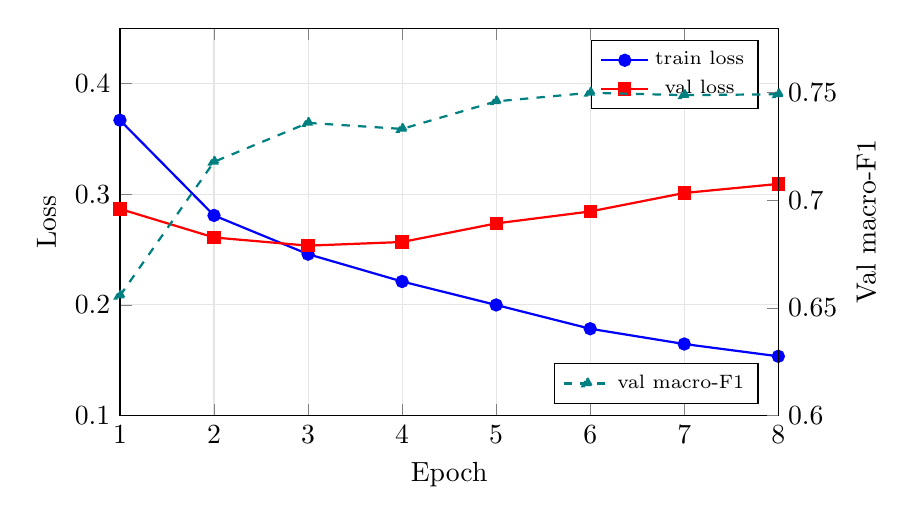
\begin{tikzpicture}
\begin{axis}[
  width=0.82\textwidth, height=6.5cm,
  xlabel={Epoch}, ylabel={Loss},
  xmin=1, xmax=8, ymin=0.1, ymax=0.45,
  legend pos=north east, legend style={font=\scriptsize},
  grid=both, grid style={gray!20},
  axis y line*=left
]
\addplot[blue, mark=*, thick] coordinates
  {(1,0.3669)(2,0.2808)(3,0.2458)(4,0.2211)(5,0.1999)(6,0.1784)(7,0.1646)(8,0.1535)};
\addlegendentry{train loss}
\addplot[red, mark=square*, thick] coordinates
  {(1,0.2867)(2,0.2609)(3,0.2535)(4,0.2568)(5,0.2736)(6,0.2844)(7,0.3011)(8,0.3093)};
\addlegendentry{val loss}
\end{axis}
\begin{axis}[
  width=0.82\textwidth, height=6.5cm,
  xmin=1, xmax=8, ymin=0.60, ymax=0.78,
  axis y line*=right, axis x line=none,
  ylabel={Val macro-F1}, ylabel near ticks,
  legend pos=south east, legend style={font=\scriptsize}
]
\addplot[teal, mark=triangle*, thick, dashed] coordinates
  {(1,0.6557)(2,0.7179)(3,0.7360)(4,0.7332)(5,0.7460)(6,0.7500)(7,0.7489)(8,0.7493)};
\addlegendentry{val macro-F1}
\end{axis}
\end{tikzpicture}
\caption{Training/validation loss (left axis) and validation macro-F1 (right
axis) over eight epochs for the deployed model (focal + label smoothing).}
\label{fig:curves}
\end{figure}

Figure~\ref{fig:bars} visualises the optimisation study, and
Figure~\ref{fig:cm} contrasts the confusion matrices of the cross-entropy
baseline and the deployed model (focal + label smoothing), making the hard-class improvement explicit.

\begin{figure}[ht]
\centering
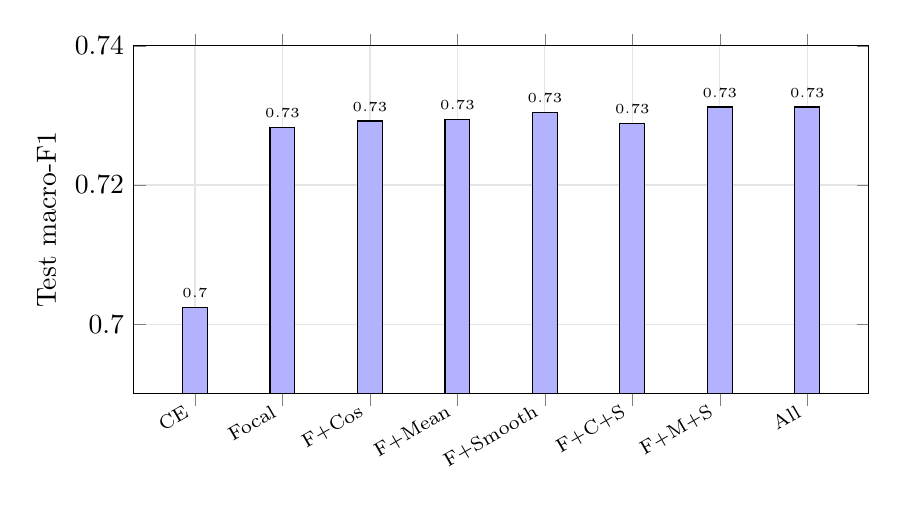
\begin{tikzpicture}
\begin{axis}[
  width=0.9\textwidth, height=6cm,
  ybar, bar width=9pt,
  ymin=0.69, ymax=0.74,
  ylabel={Test macro-F1},
  symbolic x coords={CE, Focal, F+Cos, F+Mean, F+Smooth, F+C+S, F+M+S, All},
  xtick=data, x tick label style={font=\scriptsize, rotate=30, anchor=east},
  nodes near coords, nodes near coords style={font=\tiny},
  grid=both, grid style={gray!20}
]
\addplot[fill=blue!30] coordinates
  {(CE,0.7024)(Focal,0.7283)(F+Cos,0.7292)(F+Mean,0.7294)(F+Smooth,0.7304)(F+C+S,0.7288)(F+M+S,0.7312)(All,0.7312)};
\end{axis}
\end{tikzpicture}
\caption{Test macro-F1 across the optimisation study. The cross-entropy baseline
(CE) sits clearly below the focal family; every focal configuration---single
technique or combination---then clusters in a narrow band of about 0.728--0.731,
illustrating the plateau discussed in the text.}
\label{fig:bars}
\end{figure}

\begin{figure}[ht]
\centering
% --- baseline CM ---
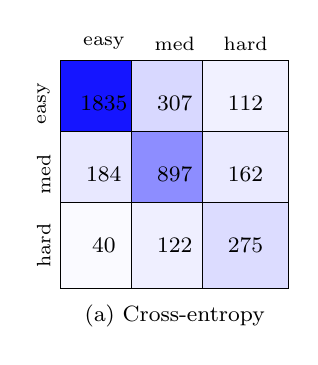
\begin{tikzpicture}[scale=0.9]
\def\cm{{1835,307,112},{184,897,162},{40,122,275}}
\foreach \row [count=\i from 0] in {{1835,307,112},{184,897,162},{40,122,275}} {
  \foreach \val [count=\j from 0] in \row {
    \pgfmathsetmacro{\shade}{min(100, \val/20)}
    \node[draw, minimum size=11mm, fill=blue!\shade] at (\j,-\i) {\footnotesize \val};
  }
}
\foreach \lab [count=\j from 0] in {easy,med,hard}
  \node[font=\scriptsize] at (\j,0.85) {\lab};
\foreach \lab [count=\i from 0] in {easy,med,hard}
  \node[font=\scriptsize, rotate=90] at (-0.85,-\i) {\lab};
\node[font=\footnotesize] at (1,-3.0) {(a) Cross-entropy};
\end{tikzpicture}
\hspace{6mm}
% --- focal+smoothing CM ---
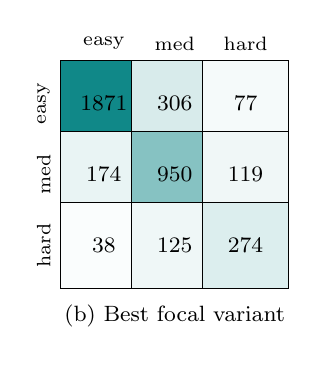
\begin{tikzpicture}[scale=0.9]
\foreach \row [count=\i from 0] in {{1871,306,77},{174,950,119},{38,125,274}} {
  \foreach \val [count=\j from 0] in \row {
    \pgfmathsetmacro{\shade}{min(100, \val/20)}
    \node[draw, minimum size=11mm, fill=teal!\shade] at (\j,-\i) {\footnotesize \val};
  }
}
\foreach \lab [count=\j from 0] in {easy,med,hard}
  \node[font=\scriptsize] at (\j,0.85) {\lab};
\foreach \lab [count=\i from 0] in {easy,med,hard}
  \node[font=\scriptsize, rotate=90] at (-0.85,-\i) {\lab};
\node[font=\footnotesize] at (1,-3.0) {(b) Best focal variant};
\end{tikzpicture}
\caption{Confusion matrices (rows = true class, columns = predicted) for the
cross-entropy baseline (a) and the deployed model, focal + label smoothing (b). Off-diagonal mass on
the hard row shrinks under the focal objective.}
\label{fig:cm}
\end{figure}

\subsection{Module Testing: Few-Shot Generation via LLM-as-a-Judge}
To test whether the difficulty-keyed few-shot bank improves question quality, the
generation pipeline was run in two conditions over five Operating-Systems content
chunks at three difficulty levels: a \emph{baseline} condition (Bloom-guided
prompt, no demonstrations) and an \emph{ICL} condition (same prompt plus
difficulty-aligned demonstrations). For each of the 15 (chunk, level) cells the
two question sets were presented to a blinded judge in randomised order, which
selected the better set per criterion. Table~\ref{tab:judge} reports how often
the ICL condition won.

\begin{table}[ht]
\centering
\caption{Blinded pairwise LLM-as-a-judge results over 15 (chunk, level) cells.
``ICL win-rate'' excludes ties.}
\label{tab:judge}
\begin{tabular}{lcccc}
\toprule
\textbf{Criterion} & \textbf{ICL wins} & \textbf{Baseline wins} & \textbf{Ties} & \textbf{ICL win-rate} \\
\midrule
Answerability       & 9 & 5 & 1 & 60.0\% \\
Constraint density  & 2 & 7 & 6 & 13.3\% \\
Difficulty match    & 9 & 6 & 0 & 60.0\% \\
Overall preference  & 9 & 6 & 0 & 60.0\% \\
\bottomrule
\end{tabular}
\end{table}

The few-shot bank is preferred on overall quality, answerability, and difficulty
match (60\% each), indicating that difficulty-aligned demonstrations help the
generator produce questions that are both solvable from the source and
appropriately calibrated to the requested level. The baseline scores higher on
\emph{constraint density}: its questions tend to enumerate many explicit options
(``which of (a), (b), (c), (d)\ldots''), inflating the count of named parameters,
whereas the ICL questions are more focused. That the judge reached different
verdicts on different criteria---rather than a single halo effect---supports the
validity of the blinded pairwise protocol.

\subsection{Integration Testing}
The two modules were exercised together by running the full generation path with
the trained classifier loaded as the inline verifier: content retrieval, example
retrieval, prompt assembly, generation, and per-question difficulty verification.
The verifier annotated each generated question with a predicted level and
confidence, and the bounded regeneration path activated when a majority of
generated questions missed the requested level, confirming that the
control-and-verify loop behaves as designed.

\section{Testing Schedule}
Testing proceeded in three stages: (1) the classifier optimisation study
(baseline followed by the focal variants), each run trained and evaluated on the
fixed data split; (2) construction and labelling of the example bank using the
deployed classifier; and (3) the blinded LLM-as-a-judge comparison of the
generation pipeline with and without the few-shot bank.

\section{Comparative Results to Previous Work}
Two findings summarise the evaluation. First, on the difficulty-classification
task, the focal objective with partial fine-tuning lifts test macro-F1 from
0.7024 to 0.7304 and, crucially, raises hard-class F1 from 0.558 to 0.604,
addressing the well-known difficulty of the highest cognitive levels noted in
prior question-generation work \parencite{scaria2024aeqg}. Stacking further
optimisations---cosine scheduling, mean pooling, label smoothing, and their
combinations---did not move the result beyond run-to-run noise (every focal
configuration lands within 0.003 of the deployed model), so we report the plain
focal model as the operating point. Second, on generation
quality, difficulty-keyed in-context demonstrations are preferred by a blinded
judge on overall quality, answerability, and difficulty match (60\% win-rate
each), consistent with the literature finding that retrieved demonstrations
improve over zero-shot prompting, and extending it by using the target difficulty
level itself as the retrieval key with an independent trained verifier in the
loop.

\printbibliography[title=References]

\end{document}
